%++++++++++++++++++++++++++++++++++++++++
% Don't modify this section unless you know what you're doing!
\documentclass[letterpaper,12pt]{article}
\usepackage{tabularx} % extra features for tabular environment
\usepackage{amsmath}  % improve math presentation
\usepackage{graphicx} % takes care of graphic including machinery
\usepackage[margin=1in,letterpaper]{geometry} % decreases margins
\usepackage{cite} % takes care of citations
\usepackage[final]{hyperref} % adds hyper links inside the generated pdf file
\hypersetup{
	colorlinks=true,       % false: boxed links; true: colored links
	linkcolor=blue,        % color of internal links
	citecolor=blue,        % color of links to bibliography
	filecolor=magenta,     % color of file links
	urlcolor=blue         
}
\usepackage{indentfirst}		% indents first paragraph
\usepackage[utf8]{inputenc} % allows usage of latin characters

%% Include color package
\usepackage[table,xcdraw]{xcolor}
\definecolor{cloudwhite}{cmyk}{0,0,0,0.025}

%% Includes source-code listings package
\usepackage{listings}
\lstset{ %
 language={},		                % choose the language of the code
 basicstyle=\footnotesize\ttfamily,
 keywordstyle=\bfseries,
 numbers=none,                      % where to put the line-numbers
 frame=tb,
 float=htb,
 aboveskip=8mm,
 belowskip=4mm,
 backgroundcolor=\color{cloudwhite},
 showspaces=false,                  % show spaces adding particular underscores
 showstringspaces=false,            % underline spaces within strings
 showtabs=false,                    % show tabs within strings adding particular underscores
 tabsize=2,	                        % sets default tabsize to 2 spaces
 captionpos=b,                      % sets the caption-position to bottom
 breaklines=true,                   % sets automatic line breaking
 breakatwhitespace=false,           % sets if automatic breaks should only happen at whitespace
 escapeinside={\%*}{*)},            % if you want to add a comment within your code
 morekeywords={*,var,template,new}  % if you want to add more keywords to the set
}

%% Enables new settings for editing tables
\usepackage{tabularx}
\newcolumntype{R}[1]{>{\raggedleft\arraybackslash}p{#1}}

%% Supports both eps and pdf files
%\usepackage{epstopdf}

\graphicspath{{figures/}}

%++++++++++++++++++++++++++++++++++++++++


\begin{document}

\begin{titlepage}
	\centering
	
\includegraphics[width=0.4\textwidth]{uporto-feup.pdf}\par\vspace{1cm}
	{\scshape\Large EEC0055\\ Projecto de Sistemas Digitais\par}
	\vspace{1.5cm}
	{\huge\bfseries Laboratory 3: All-digital FM stereo modulator\par}
	\vspace{2.5cm}
	{\Large João Beleza, Pedro Costa\par}
	\vspace{0.25cm}
	{\{up201402831, up201402793\}@fe.up.pt\par}
	\vfill

	\vfill

	{\large \today\par} % bottom of the page
\end{titlepage}

\section{System overview}

This report provides information on an all-digital FM stereo modulator developed as a final project for Projecto de Sistemas Digitais. 

A general overview of the project and its sub-modules can be seen in \autoref{fig:overview}.

\begin{figure}[!h]
\centering
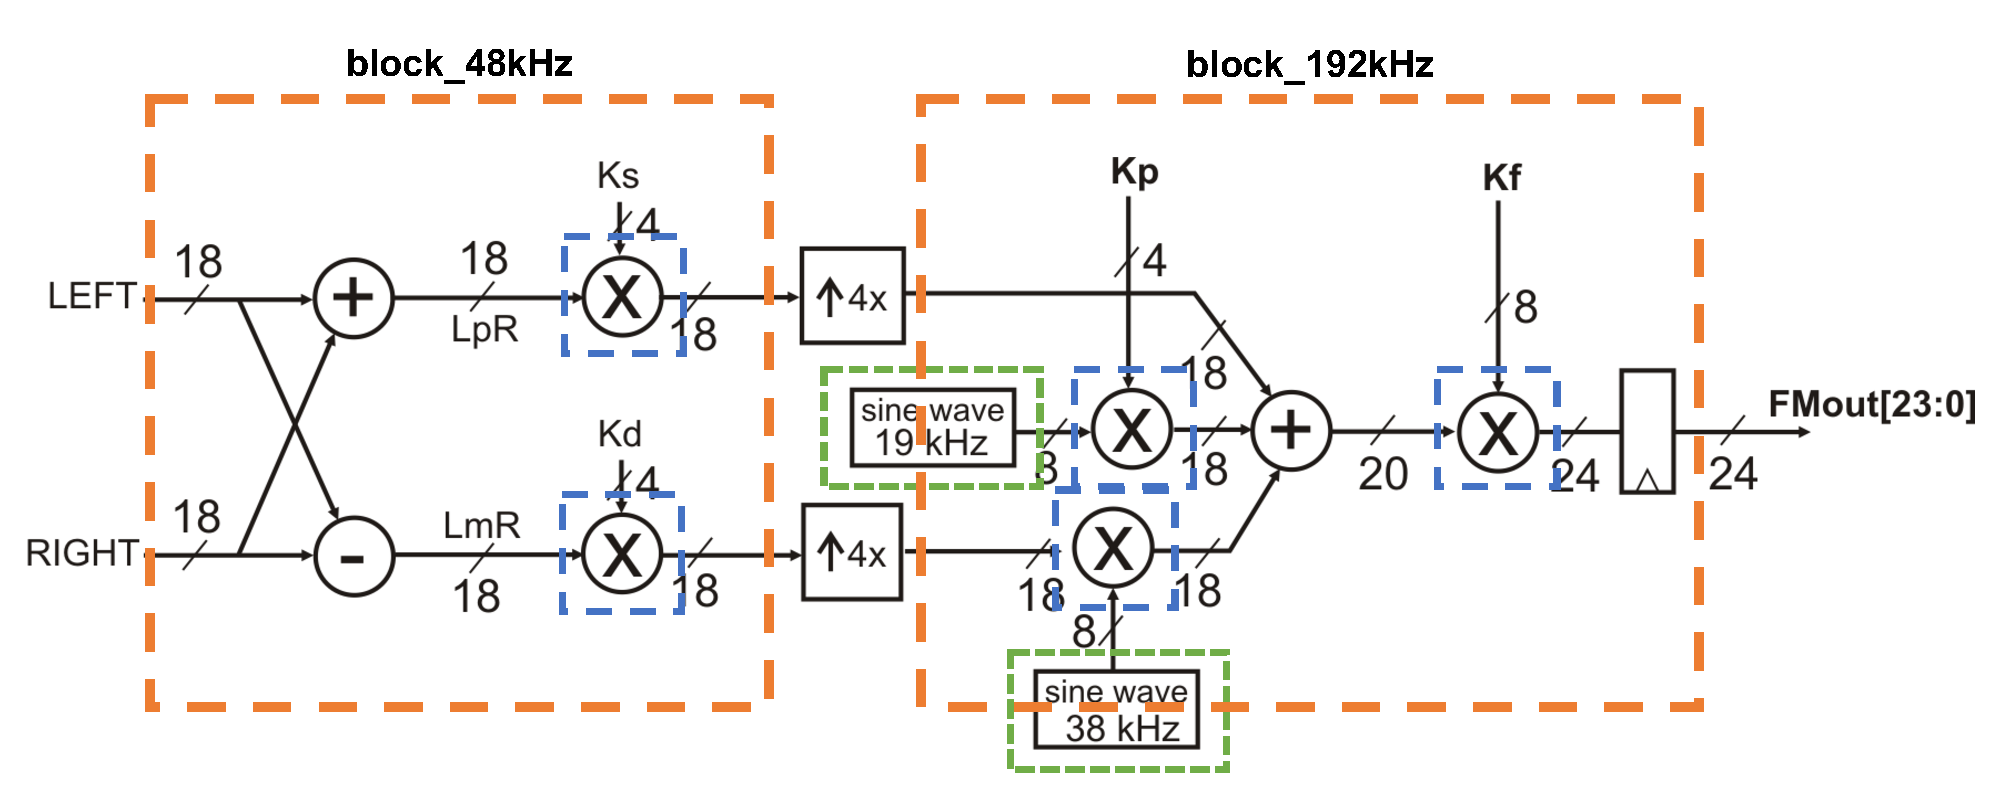
\includegraphics[width=0.7\textwidth,height=0.2\textheight]{overview.pdf}
\caption{Block diagram overview of the project. Implemented macro blocks are highlighted in orange; DDS blocks are seen in green; improved multiplication blocks are seen in blue.}\label{fig:overview}
\end{figure}

The implementation of this project was wrapped under a single module named \texttt{my\_fm\_module}, which was split into the following blocks:

\begin{itemize}
	\item \texttt{block\_48kHz}: corresponds to the leftmost block, which receives the stereo input at a sample rate of 48 kHz. Its outputs will feed each of the interpolators.
	\item \texttt{interpol\_4x}: interpolate the signal for further processing. The blocks used were provided as IP blocks.
	\item \texttt{block\_192kHz}: corresponds to the rightmost block, which processes the signal at a rate of 192 kHz. It outputs the final FM signal.
\end{itemize}

Besides this, two additional modules were implemented:
\begin{itemize}
	\item \texttt{dds}: implements each of the sine wave generators. Implementation details can be read in \autoref{sec:dds-module}.
	\item \texttt{seqmultNM\_sat}: implements a wrapper of the original \texttt{seqmultNM} IP block. It implements some of the control logic detailed in \autoref{sec:control-path}, as well as a comprehensive mechanism that allows for rescaling the number and for saturating the output, thus avoiding overflow.
\end{itemize}

All sums and shifting operations were performed using standard Verilog code.

Furthermore, some optimisations were performed throughout the implementation of the project. These are described under \autoref{sec:further-optimisations}.


\section{DDS module}\label{sec:dds-module}

In this section, the DDS (Direct Digital Synthesiser) modules implemented in the project will be discussed.

Below follows the implementation used in the final version of the project:
\begin{lstlisting}[caption=Pseudo-code for final DDS implementation]
	* Parameter definitions are used for
		- NBITS_PHASE: # of bits of phase
		- NBITS_PHASE_FRAC: # of bits of fractionary part of phase
		- NSAMPLES_LUT: # of samples used in the LUT (Lookup Table)
		- HEXVAL: string containing the path for the values to be inserted in the LUT
	* Values are uploaded from the file to the LUT using $readmemh()
	* With posedge clock, if reset is not active:
		- if enableclk input is active, then phase must be updated
		- outsine output is updated in accordance with the latest value of phase
\end{lstlisting}

Besides this, a second DDS implementation was developed with the purpose of reducing the final circuit size. To achieve this, a module taking advantage of the periodicity properties of the wave, shown in \autoref{fig:sine-matlab}, was implemented.

\begin{figure}[!h]
\centering
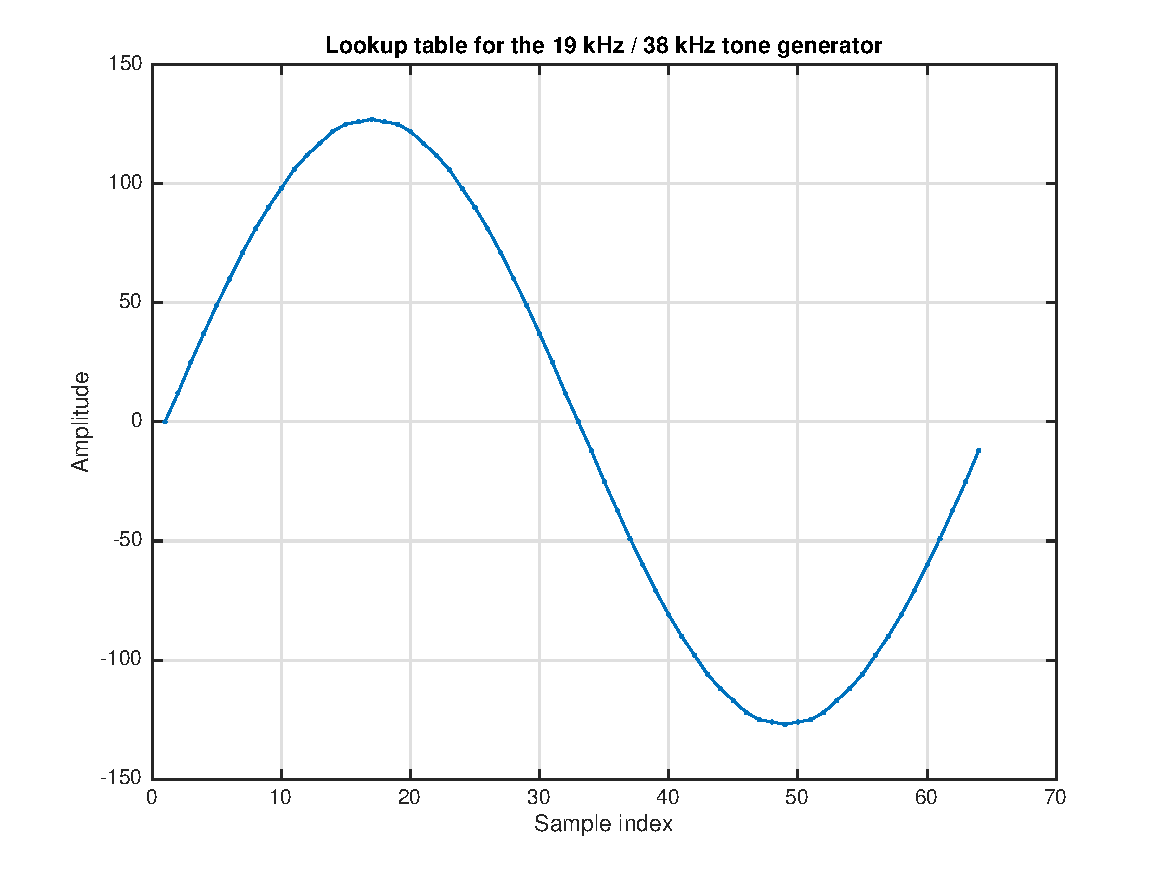
\includegraphics[width=0.7\textwidth]{sine-matlab.pdf}
\caption{Sine wave waveform and LUT values}\label{fig:sine-matlab}
\end{figure}

%% Não esquecer de falar sobre os erros corrigidos na bench do prof 8)

Because the number of samples of the LUT is a power of two, it is possible to infer the complete signal by only storing a fraction of the signal. This allowed for a reduction of the size of the LUT by 75\%. Upon further testing, it was verified that this implementation provides for area optimisations. Among others, the number of block RAM/FIFO was reduced from 1 to 0 (as seen in \autoref{table:device-utilisation}).

The module was implemented as follows:

\begin{lstlisting}[caption=Pseudo-code for an optimised implementation of the DDS]
	* Parameter definitions are used for
		- NBITS_PHASE: # of bits of phase
		- NBITS_PHASE_FRAC: # of bits of fractionary part of phase
		- NBITS_OUTPUT: # of bits in the output
		- NSAMPLES_LUT: # of samples used in the LUT (Lookup Table)
		- HEXVAL: string containing the path for the values to be inserted in the LUT
	* Values are uploaded from the file to the LUT using $readmemh()
	* sineLUT_i variable is assigned to translate the previously used phase logic to a logic that supports a smaller LUT
	
	* With posedge clock, if reset is not active:
		- if enableclk input is active, then phase must be updated
		- if value of phase equals NSAMPLES_LUT/4, sine output equals to the maximum representation value
		- if value of phase equals 3*NSAMPLES_LUT/4, sine output equals to the minimum representation value
		- else, if phase[NBITS_PHASE-1] (the MSB for phase representation is enabled), then values should be output from the LUT as negative
		- else, values should be output as is from the LUT
\end{lstlisting}















\section{Control path}\label{sec:control-path}

In this section the control path will be explained, followed by the implementation of both \texttt{block\_48kHz} and \texttt{block\_192kHz} blocks. These are an application of that same algorithm.

The multiplication block is essential for the correct functioning of the system. As such, the control path was designed around its requirements, as detailed below.

\begin{lstlisting}[caption={Description of the control path}, label={lst:control}]
	* Start phase:
		- The inputs are continually updated in accordance with each multiplier
		- The start flag of the multiplier is enabled
	* Multiplier phase:
		- The control flag is enabled when the ready flag is low
	* Final phase:
		- Results are signalled as ready when both control and ready flags are enabled
		- Upon acknowledging the valid results, the control flag is set to low
\end{lstlisting}

\subsection{block\_48kHz}

For this block, both inputs are being added and subtracted continuously by means of an \emph{assign} condition. Any possible overflow is avoided by discarding the LSB as a result of a previous sum which preserves any overflow information.

Due to requirements of the \texttt{seqmultNM} blocks, both \texttt{Ks} and \texttt{Kd} gains are extended by a signal bit, so as to be interpreted as signed (and positive) variables.

The multiplier is enabled using the signal \texttt{clocken\_48}, which is active during a single clock cycle, with a periodicity of 48 kHz. After this, the strategy in \autoref{lst:control} is used, and its output is directed to the inputs of the \texttt{interpol4x} blocks. Using the \texttt{seqmultNM\_sat} described under \autoref{sec:further-optimisations}, the outputs of both multipliers are shifted by 3 bits to the right.

\subsection{block\_192kHz}

For this block, a similar implementation is performed. The gains \texttt{Kp} and \texttt{Kf} are extended by a signal bit. The output of both \texttt{dds} blocks is placed in a 8-bit register. 

The multipliers at the left of the sum block (see \autoref{fig:overview}) are enabled using the signal \texttt{clocken\_192}, which is active during a single clock cycle, with a periodicity of 192 kHz. Besides this, a condition is added, which signals that all calculations are finished within the block. For the multiplication with the 38 kHz sine wave, the result is affected by an 8-bit right shift. For the multiplication with the 19 kHz sine wave, the result is affected by an 6-bit left shift. Both outputs are rescaled using the \texttt{seqmultNM\_sat} block.

A single \emph{assign} statement is used for the summation of all three values before the rightmost multiplication. When both multiplications before this sumation finishes, as described under \autoref{lst:control}, the results are acknowledged. This disables the flags of the multipliers on the left of the summation, and enables the rightmost multiplication. Its output already counts for a 4-bit shift. A control flag is enabled, which states that all calculations are finished, and its values are loaded into a registered output with a periodicity of 192 kHz.


\section{Further optimisations}\label{sec:further-optimisations}

\subsection{Architectural optimisations}

In order to optimise the circuit, a minimum area target was defined.

To achieve this, some strategies were followed, as is explained below.

\subsubsection*{Coding}

Below are listed the performed optimisations:
\begin{itemize}
	\item Definition of \texttt{seqmultNM} blocks with \texttt{N} (multiplier) having the most bits and \texttt{M} (multiplicand) having the least bits. This increases the number of cycles needed for computation (but still manages to meet timing constraints), but allows for decreases in area
	\item Elimination of all duplicate \texttt{reg} and \texttt{wire} instantiations
\end{itemize}

Further optimisation was also attempted. However, some measures didn't translate into additional optimisation gains. The attempted procedures are listed below:
\begin{itemize}
	\item Condensation of all division and multiplication scenarios in \texttt{seqmultNM\_sat} by using a \emph{wire} assignment before comparing the final value
	\item Utilisation of \texttt{else ... if} statements when in the presence of mutually exclusive statements (e.g. \texttt{x} versus \texttt{!x})
	\item Utilisation of registers to save all previous inputs from multipliers, in order to lower power consumption in case the results remained unaltered (removed due to increase in area size)
	\item Utilisation of two-step sum in \texttt{block\_192kHz} (i.e. by performing two sums with two operands instead of a single sum with three operators
\end{itemize}

\subsubsection*{Synthesis}
After validation of the final design, synthesis optimisation was achieved by means of editing the \texttt{Optimisation Goal} and \texttt{Optimisation Effort} parameters under the \texttt{Synthesis - XST > Process Properties} options.

Maximum optimisation was achieved using the values listed below. The resulting device utilisation statistics are presented in \autoref{table:device-utilisation}.

\begin{table}[!h]
\center
\begin{tabular}{|p{6cm}|p{2cm}|}
\hline
\textbf{Optimisation Goal}   & Speed  \\ \hline
\textbf{Optimisation Effort} & Normal \\ \hline
\end{tabular}
\end{table}

\subsection{Resource occupancy}

The results for the resource occupancy of the device upon synthesis follow below.

%Having the clock frequency fixed to \emph{insert\_freq\_here}, 
\begin{table}[!h]
\center
\begin{tabular}{|l|R{2.25cm}|R{2.25cm}|R{2.25cm}|}
\hline
\rowcolor[HTML]{FFFF99} 
\textbf{Logic utilisation}        & \multicolumn{1}{l|}{\cellcolor[HTML]{FFFF99}\textbf{Used}} & \multicolumn{1}{l|}{\cellcolor[HTML]{FFFF99}\textbf{Available}} & \multicolumn{1}{l|}{\cellcolor[HTML]{FFFF99}\textbf{Utilisation}} \\ \hline
Number of Slice Registers         & 1732                                                       & 54576                                                           & 3\%                                                               \\ \hline
Number of Slice LUTs              & 1319                                                       & 27288                                                           & 5\%                                                               \\ \hline
Number of fully used LUT-FF pairs & 898                                                       & 1778                                                            & 50\%                                                              \\ \hline
Number of bonded IOBs             & 78                                                         & 218                                                             & 35\%                                                              \\ \hline
Number of Block RAM/FIFO          & 0                                                          & 116                                                             & 0\%                                                               \\ \hline
\end{tabular}
\caption{Device utilisation results for the final optimised synthesis}\label{table:device-utilisation}
\end{table}

\subsection{Additional changes}

Besides this, a change was performed to the FM stereo data generation data generation script (\texttt{fmstereo\_gensimdata.m}). An imprecision was detected in lines 135 and 137, in which the generated data, when saturating to a negative value, would exceed the representation range of the hardware, a wrong value. The code was changed so as to saturate to the most negative value possible to represent by its number of bits.


\end{document}
